\section{Theoretische Hintergründe}

\subsection{Einordnung und Abgrenzung zu anderen Algorithmen} \label{chap:Einordnung}

Der Ant Colony Algorithmus gehört zu den metaheuristischen Optimierungsverfahren. Hierzu wird eine abstrakte Folge von Schritten  definiert, die anschließend auf eine Problemstellung angewandt werden soll. Jeder einzelnen Schritt sollte hierbei jedoch problemspezifisch implementiert werden. Die Anwendung findet vor allem bei schweren kombinatorischen Optimierungsproblemen statt, für die es noch keinen anderen effizienten Lösungsalgorithmus gibt. Es wird in der Metaheuristik versucht einen Suchalgorithmus zu finden, der bei vollständigen oder unvollständigen Informationen eine optimale Lösung liefert. \newline
Wenn die Metaheuristik weiter klassifiziert wird, erhält man folgende Varianten:

\begin{itemize}
  \item local search vs global search
  \item single solution vs population based
  \item von der Natur inspirierte Metaheuristik
  \item von der Antiken inspirierte Metaheuristk
\end{itemize}

Der Ameisenalgorithmus gliedert sich unter global search und population based Algorithmus ein. 
Das Verhalten solcher Algorithmen basiert entsprechend auf dem Verhalten von verschiedenen Schwärmen wie beispielsweise von Vögeln, Fischen oder Insekten. Hierzu wird das Verhalten der Lebewesen bei der Futtersuche analysiert und versucht auf ein reales Problem anzuwenden. Ein weiteres schwarmbasierte Optimierungsverfahren aus der Natur umfasst die Partikelschwarmoptimierung. Hier wird jedoch anders wie bei Ameisenalgorithmus versucht, eine Kandidatenlösung bezogen auf ein Qualitätsmaß zu erhalten. 

\subsection{Verhalten von Ameisen bei der Futtersuche}\label{chap:VerhaltenAmeisen}
Ameisen haben eine eigene Verhaltensweise bei Ihrer Futterbeschaffung. Zwischen Ameisenhaufen und Futter besteht eine direkte Ameisenstraße. Mittels einer Drüse die die Ameisen am hinteren Teil Ihres Körpers haben, können die kleinen Insekten einen Lockstoff, auch Pheromon genannt, ausschütten. Nachdem eine Ameise einen bestimmten Weg gelaufen ist, liegt dementsprechend entlang des Weges die genannte Pheromonspur zugrunde. Nachfolgende Ameisen können sich genau an dieser Pheromonspur orientieren um den selben Weg wie die Vorgängerameise zu nehmen. Die Ameisen orientieren sich stehts an dem Weg, bei dem die größte Pheromonspur vorliegt. Dies ist vorteilhaft da zwischen Ameisenhaufen und Futterquelle meistens mehrere mögliche Wege liegen können. Es wird somit garantiert dass die Ameisen stehts einer der kürzeren Wege nehmen. Bei der ersten Futtersuche schwärmen die Ameisen in unterschiedliche Richtungen aus. Sollten beispielsweise zwei Ameisen auf unterschiedlichen Wegen zu einer Futterquelle gelangen, würde diejenige Ameise die den längeren Weg hat, den Rückweg der schnelleren Ameise nehmen, da dieser Weg bereits eine doppelte Pheromonspur aufweist. Der eigene Weg der Ameise  würde im Gegensatz dazu lediglich eine einfache Pheromonspur aufweisen. Dadurch kann festgehalten werden, je öfter Ameisen einen Weg gehen, desto größer ist die Pheromonspur. Der Nachteil dieser Eigenschaft liegt darin, dass ein möglicher kürzerer Weg von keiner Ameise genommen wird, da auch keine Pheromonspur vorliegt. Die dargestellten Informationen wurden von Nahrstedt \citep[S.213-214]{Nahrstedt.2018} entnommen.\newline
Diese Vorgehensweise der Ameisen wird im Shiny Dashboard mittels einer Slide-Show dargestellt. Es wurden zusätzlich drei InfoButtons programmiert, die dem User zusätzliche Informationen zu den drei aufgestellten Phasen geben sollen.
\newline
- Phase 1 Orientierung: beschreibt wie die Ameisen sich bei der Suche einer neuen Futterquelle verhalten
\newline
- Phase 2 Routine: beschreibt wie sich die Ameisen bei einer gefundenen Futterquelle bezüglich der Pheromone verhalten.
\newline
- Phase 3 Dauerhaftigkeit: beschreibt dass trotz möglichen kürzeren Wegen, trotzdem der mit den meisten Pheromonen behafteteste Weg gewählt wird.
\newline
Die UI Funktion für das Einbetten der Slideshow und der drei Infobuttons wird in Abb. \ref{fig:ui_ant_foraging_tab} und die Server Funktion in Abb. \ref{fig:server_ant_foraging_tab} dargestellt.

\begin{figure}[h]
 \centering
 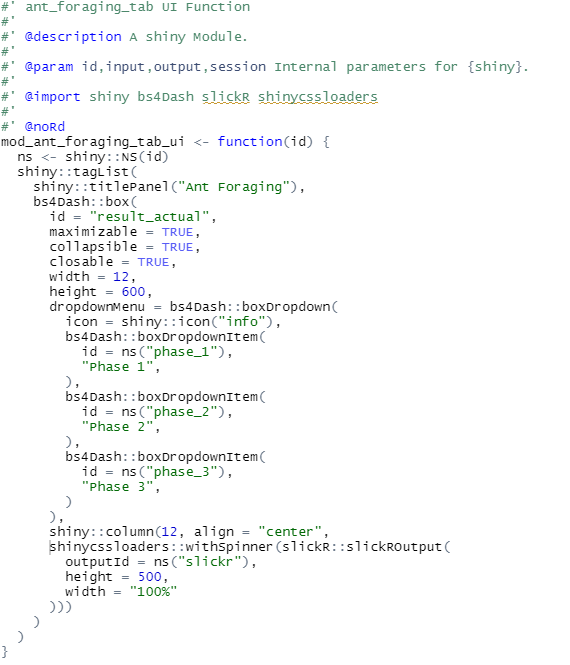
\includegraphics[scale=.6]{"images/03_Theoretische_Hintergründe/ui_ant_foraging_tab.png"}
 \caption{Quellcode für die UI Funktion der Slideshow}
 \label{fig:ui_ant_foraging_tab}
\end{figure}

\begin{figure}[h]
 \centering
 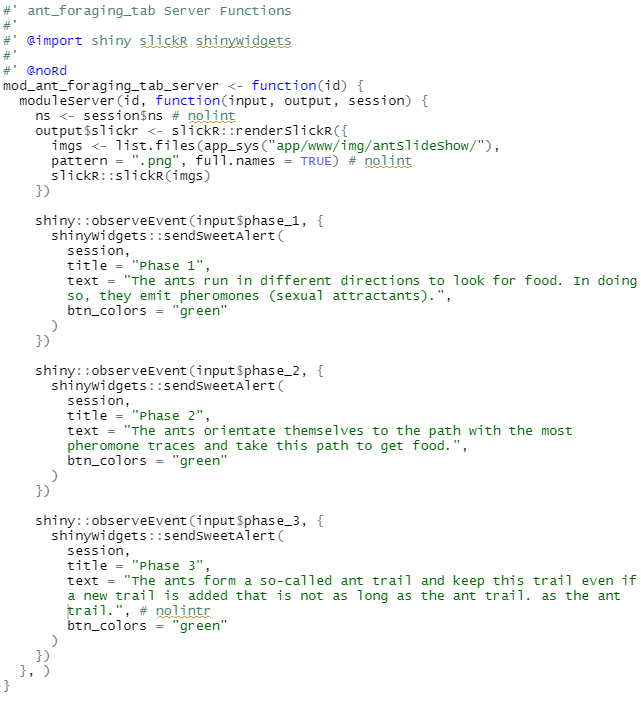
\includegraphics[scale=.6]{"images/03_Theoretische_Hintergründe/server_ant_foraging_tab.png"}
 \caption{Quellcode für die Server Funktion der Slideshow}
 \label{fig:server_ant_foraging_tab}
\end{figure}

Um dem User das Verhalten der Ameisen bei der Futtersuche näherzubringen wurde eine Slide Show integriert, die eine Vielzahl von Bildern enthält. Die Bilder zeigen die einzelnen Schritte des Verhaltens der Ameisen. Die SlideShow funktioniert wie eine Art Karussel. Man startet mit dem ersten Bild und geht reihum zu dem jeweiligen nächsten Bild, bis man beim letzten Bild angelangt ist. Nachdem beim letzten Bild auf weiter gedrückt wird, kommt man wieder zum ersten Bild.
Es wurde zusätzlich zur Slideshow ein Spinner ergänzt, um dem User bei eventuellen Wartezeiten im Dashboard eine Ladeanimation anzuzeigen. Der verwendete Code wurde angelehnt an dem Codebeispiel unter  \href{https://stackoverflow.com/questions/51531743/image-slideshow-in-r-shiny}{stack overflow} implementiert.

\subsubsection{Übertragung des Verhaltens von Ameisen auf Algorithmen} \label{chap:Formeln}
Mit dem Prinzip von Ameisen bei der Futtersuche lassen sich Optimierungsprobleme wie beispielsweise die Suche nach dem kürzesten Pfad zwischen zwei Punkten lösen. Mathematisch wird dies umgesetzt, indem künstliche Ameisen instanziiert werden, ihre Ergebnisse berechnet werden, eine Gesamtlösung aus den Lösungen der einzelnen Ameisen gebildet wird und die Pheromonkonzentration der Pfad-Abschnitte aktualisiert wird. Dieser Ablauf wird wiederholt bis das Ergebnis zufriedenstellend ist oder ein Abbruchkriterium erreicht ist. Beispielsweise könnte letzteres so definiert sein, dass abgebrochen werden kann, sobald sich das Gesamtergebnis der Ameisen innerhalb von zwanzig aufeinanderfolgenden Iterationen nicht mehr ändert.\citep{Pyl2008} \newline
    Die Formeln, die auf dem R-Shiny Dashboard dargestellt werden, beziehen sich auf den ursprünglichen Ameisenalgorithmus Ant System. Die Formeln der Erweiterungen und Weiterentwicklungen des Algorithmus Ant System werden nicht dargestellt, um den Betrachter des R-Shiny Dashboard nicht zu überfordern und die Komplexität nicht zu erhöhen. Die dargestellten Informationen wurden \cite{Pyl2008} sowie \cite[S. 20-30]{Graf.2003} entnommen. 

\begin{figure}[h]
 \centering
 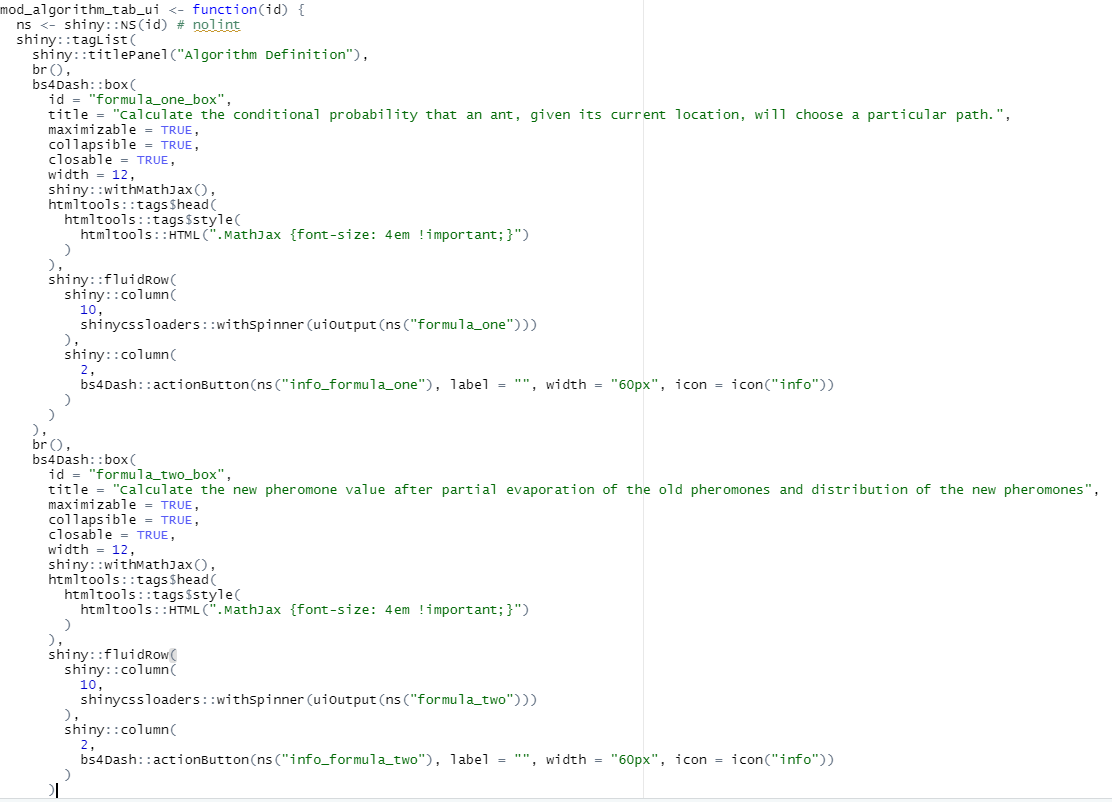
\includegraphics[scale=0.6]{"images/03_Theoretische_Hintergründe/ui_Formeln.png"}
 \caption{Ausschnitt des Quellcodes der ui-Funktion des Moduls mod\_algorithm\_tab zur Darstellung der Formeln des ACO}
 \label{fig:formeln_ui}
\end{figure}

Die Datei mod\_algorithm\_tab.R beinhaltet den für dieses Kapitel erstellten Quellcode.
Abbildung \ref{fig:formeln_ui} zeigt drei Output-Elemente der ui-Funktion, für die Darstellung von drei mathematischen Formeln und drei Infobuttons, die Erläuterungen zu den Formeln auf Knopfdruck anzeigen lassen sollen.

\begin{figure}[h]
 \centering
 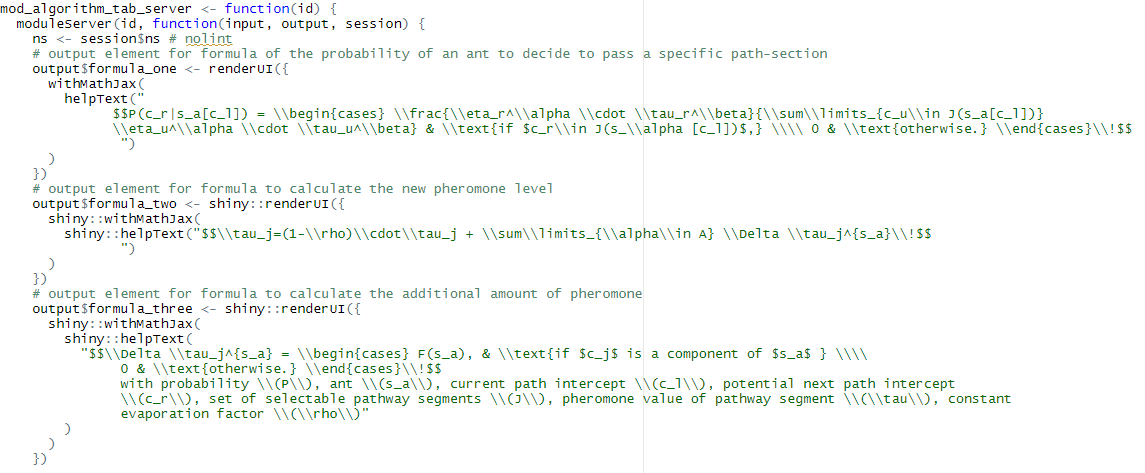
\includegraphics[scale=0.6]{"images/03_Theoretische_Hintergründe/server_Formeln_1.png"}
 \caption{Ausschnitt des Quellcodes der Server-Funktion des Moduls mod\_algorithm\_tab zur Darstellung der Formeln des ACO}
 \label{fig:formeln_server_1}
\end{figure}

Abbildung \ref{fig:formeln_server_1} zeigt wie die Formeln in der mithilfe der Bibliothek MathJax dargestellt werden. Nach der letzten Formel wird außerdem die Bedeutung der Formelzeichen angegeben. Der Aufbau der output-Elemente ist bei allen Formeln derselbe. 
Im Quellcode auf Abbildung \ref{fig:formeln_server_2} werden Aktionen für die Informations-Buttons definiert. Jeder der Buttons löst ein Pop-up-Fenster aus, in dem erläuternde Informationen zur jeweiligen Formel dargestellt werden.

\begin{figure}[h]
 \centering
 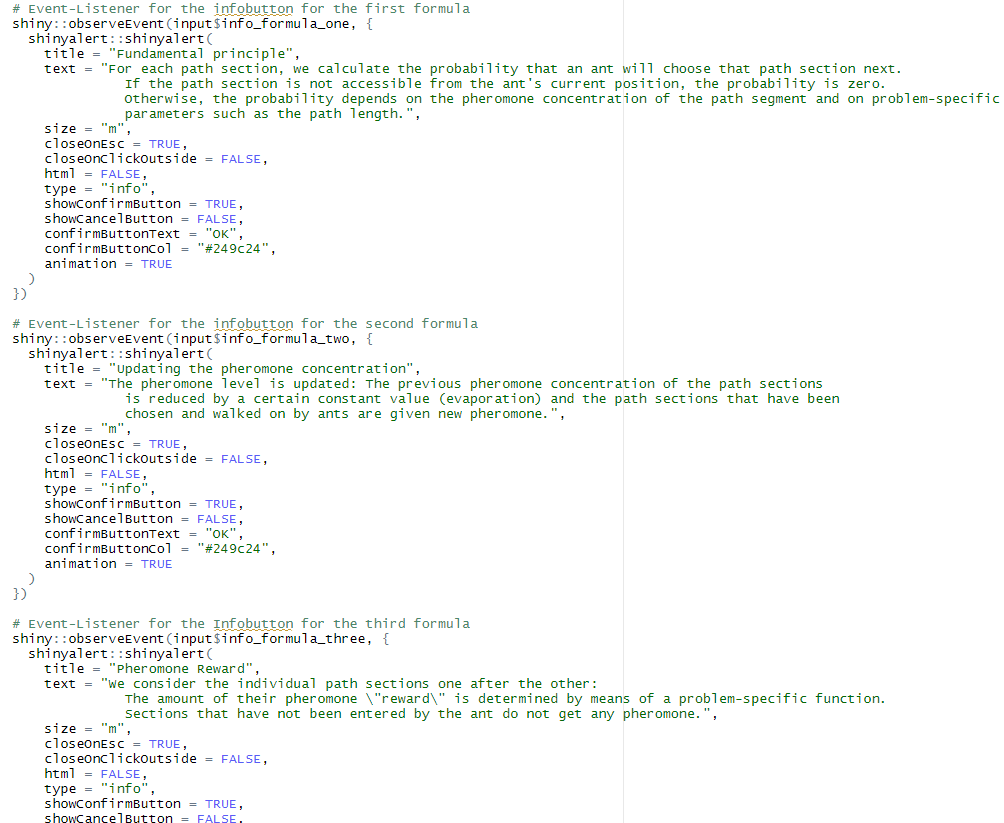
\includegraphics[scale=0.6]{"images/03_Theoretische_Hintergründe/server_Formeln_2.png"}
 \caption{Ausschnitt des Quellcodes der server-Funktion des Moduls mod\_algorithm\_tab zur Aktionsausführung der Infobuttons zur Erklärung der Formeln des ACO}
 \label{fig:formeln_server_2}
\end{figure}

Mithilfe der ersten, dargestellten Formel wird die Wahrscheinlichkeit, dass sich die Ameise für einen gewissen Pfad-Abschnitt entscheidet, berechnet. Dies hängt im wesentlich von der Pheromonkonzentration auf dem jeweiligen Pfad-Abschnitt und einem Parameter, der problemspezifisch gewählt werden kann, ab.
Mithilfe der zweiten Formel werden die Pheromonkonzentrationen aktualisiert. Hierzu gehört die Verdunstung, d.h. Verringerung des Pheromons aller Pfad-Abschnitte um einen bestimmten Anteil und die Verteilung von neuem Pheromon auf den im letzten Iterationsschritt von Ameisen begangenen Pfad-Abschnitten. 
Die letzte Formel stellt dar, wie die Verteilung von neuem Pheromon vollzogen wird. 
\newline 
Wie gut das Ergebnis des Algorithmus ist, hängt von der Parameterwahl und der problemspezifischen Implementierung ab. Um geeignete Parameter zu finden, muss häufig \glqq herumprobiert\grqq{} werden, da es keine allgemeine Methode gibt, um diese optimal zu bestimmen.
Gemäß \citet{Pyl2008} funktionieren Ameisenalgorithmen in der Praxis  oft sehr gut und sie können Mängel der klassischen Optimierungsverfahren ausgleichen.

\subsubsection{Geschichte, Entwicklung und Herkunft} \label{chap:Geschichte}
Der Ameisenalgorithmus wurde schon 1940 von dem Physik-Nobelpreisträger Richard P. Feynman betrachtet und hat in einem seiner Bücher beschrieben, wie sich die Ameisen bei der Futtersuche verhalten. Entwickelt wurde der erste Ameisenalgorithmus für Optimierungsprobleme 1991 von Colorni, Dorigo und Maniezzo. Dieser wurde damals auf das Problem des Handelsreisenden angewandt, dafür wurde der Ant System Algorithmus verwendet. Der Algorithmus wurde in den folgenden Jahren immer weiterentwickelt und 1997 kam das Ant Colony System von Luca Maria Gamberdella und 1999 das Max-Min Ant System von Thomas Stützle an die Öffentlichkeit. 
\newline
Im Laufe der Zeit wurden immer mehr verschiedenen Ameisenalgorithmen entwickelt, um die Probleme der früheren Lösungen zu verbessern oder um einen Ameisenalgorithmus spezifisch für die verschiedenen Optimierungsprobleme anwenden zu können \citep[S.5-11]{Blum2003}.
\begin{itemize}
  \item Ant System
  \item Ant Colony System
  \item Ant System mit „Elitist Strategy“
  \item Ranke Based Version von Ant System
  \item Hybrid Ant System
  \item Max-Min Ant System
  \item Approximate Nondeterministic Tree Search
  \item Fast Ant System
\end{itemize}

Wie der Name schon sagt, wurde der Algorithmus von dem natürlichen Verhalten der Ameisen in der Natur abgeschaut. Obwohl die Ameisen in einer Kolonie relativ simplen Verhaltensweisen folgen, schaffen sie es komplexe Probleme zu bewältigen. Es wurde betrachtet, wie die Ameisen sich bei der Futtersuche verhalten. Die meisten kennen das Phänomen der Ameisenstraße, die sich bildet, wenn die Ameisen Futter gefunden haben und viele Ameisen einer Kolonie das Futter holen möchten. Die Bildung dieser Straße und wie sie sich aus einem Irrweg entwickelt, wurde betrachtet und als Algorithmus versucht darzustellen \citep[S.1-4]{Blum2003}.
\newline
\newline
Bei der Futtersuche gehen die Ameisen verschiedene Wege zu der Futterquellen und hinterlassen konstant eine Pheromonspur. Mit diesem Geruch können die Ameisen unterscheiden, welchen Weg sie gelaufen sind. Laufen mehr Ameisen den gleichen Weg wird die Spur immer stärker. Ameisen laufen automatisch immer die stärkste Spur ab, da sie wissen, dass auch viele andere Ameisen diese Spur nehmen und sie daher ein guter Weg zu ihrem Ziel darstellt. Gehen zwei Ameisen unterschiedliche Wege zu einer Futterquelle, bekommt der Weg der Ameise, die schneller bei der Quelle ist, einen stärkeren Geruch, da sie den Weg schneller ein zweites Mal bestreut. Die anderen Ameisen im Nest, erkennen nun an der Spur, dass der Weg dieser Ameise schneller ist und laufen diesen nach. Hier kommt vor allem eine Entwicklung des Ant Colony System gegenüber dem Ant System zum Vorschein. Die Pheromonspur verblasst bei dem Ant Colony System langsam, dadurch ist es für die Ameisen möglich neue Wege und auch bessere Wege zu entdecken \citep[S.33-35]{OKWU.2021}.
\newline